\documentclass[11pt]{standalone}
\usepackage{amssymb} 
\usepackage{amsmath} 
\usepackage[no-math]{fontspec}
\usepackage{unicode-math}
\setmainfont{TeX Gyre Heros}
\setmathfont{Stix Two Math}
\usepackage{xcolor}
\usepackage{tikz}
\usetikzlibrary{arrows.meta, backgrounds}
\definecolor{myblue}{HTML}{005A94}
\definecolor{lightblue}{HTML}{BFDBFE}
\definecolor{bgcolor}{HTML}{E5E7EB}
\definecolor{highlight}{HTML}{CCDEE9}
\begin{document}
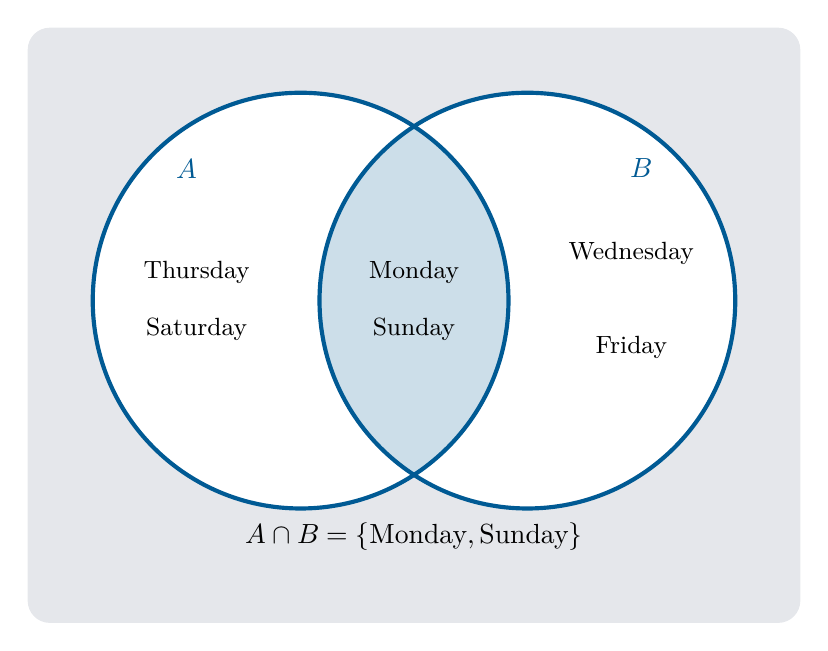
\begin{tikzpicture}[scale=1.2,
    show background rectangle,
    background rectangle/.style={fill=bgcolor, rounded corners=8pt},
    inner frame sep=0.8cm
]
  
  % Menge A (linker Kreis)
  \begin{scope}
    %\clip (1.2,0) circle (2.2cm);
    \fill[white] (-1.2,0) circle (2.2cm);
  \end{scope}
  
  % Menge B (rechter Kreis)
  \begin{scope}
    %\clip (-1.2,0) circle (2.2cm);
    \fill[white] (1.2,0) circle (2.2cm);
  \end{scope}
  
  % Schnittmenge (Überlappung) hervorheben
  \begin{scope}
    \clip (-1.2,0) circle (2.2cm);
    \fill[highlight] (1.2,0) circle (2.2cm);
  \end{scope}
  
  % Kreise zeichnen
  \draw[thick, draw=myblue, line width=1.5pt] (-1.2,0) circle (2.2cm);
  \draw[thick, draw=myblue, line width=1.5pt] (1.2,0) circle (2.2cm);
  
  % Labels für die Mengen
  \node[myblue, font=\bfseries] at (-2.4,1.4) {$A$};
  \node[myblue, font=\bfseries] at (2.4,1.4) {$B$};
  
  % Elemente in A \ B
  \node[font=\small] at (-2.3,0.3) {Thursday};
  \node[font=\small] at (-2.3,-0.3) {Saturday};
  
  % Elemente in A ∩ B (Schnittmenge)
  \node[font=\small] at (0,0.3) {Monday};
  \node[font=\small] at (0,-0.3) {Sunday};
  
  % Elemente in B \ A
  \node[font=\small] at (2.3,0.5) {Wednesday};
  \node[font=\small] at (2.3,-0.5) {Friday};
  
  % Formel
  \node at (0,-2.5) {$A \cap B = \{\text{Monday}, \text{Sunday}\}$};
  
\end{tikzpicture}
\end{document}
